\chapter{Developer Documentation}

In this chapter we aim to describe the implementation of the demo version of our game.
In the first section~\ref{sec:docs-proj} we describe the overall structure, and in the later sections we go into more detail about the individual parts.
Section~\ref{sec:docs-data} describes what goes on from the application start to the end, including all procedural generation, but not what happens during a battle.
We will focus on battles first, in section~\ref{sec:docs-battle}.

\section{Project Structure}\label{sec:docs-proj}

In Unity, each project is composed of individual scenes.
The scenes contain game objects to which are attached scripts that provide their behavior.
These are all saved in the project's asset folder, along with all other resources like prefabs, models, materials, textures, sounds and more.
They are separated to folders based on their type, for example all scenes are in the \emph{Scenes} folder.

In addition to the project assets, an important part of the project are the project settings.
However, these are all mostly set to their default value from the standard \emph{3D (Built-in render pipeline)} project template.
The settings that were changed are all uninteresting adjustments that an experienced Unity user would expect us to configure how we did, based on the explanation of our project provided in this chapter and chapter~\ref{analysis}.
These include for example settings in categories \emph{Tags and Layers}, \emph{Physics} and \emph{Player}.

\subsection{Scenes}\label{sec:docs-scenes}

The demo version of our game is composed of 5 scenes.
We provide a brief summary of each, but we will describe them in more detail later.
This summary will be useful for the rest of the chapter, allowing us to see which parts of the game occur chronologically after other parts.
For convenience, the transitions between the scenes are shown in figure~\ref{fig:scene-transitions}.

\begin{center}
    \captionsetup{type=figure}
    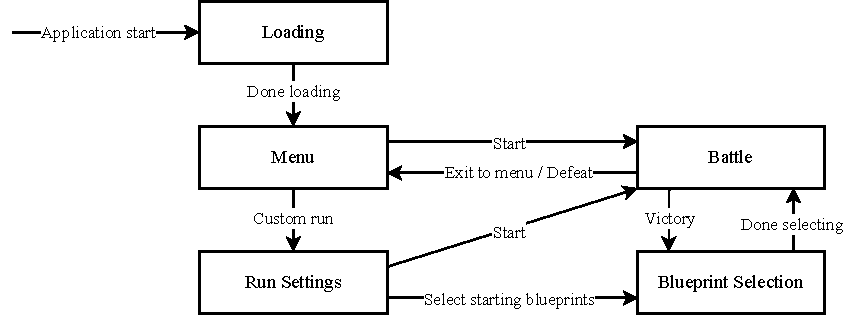
\includegraphics[width=0.9\textwidth]{img/Scene transitions.pdf}
    \caption{Scene transitions.}
    \label{fig:scene-transitions}
\end{center}

\begin{itemize}
    \item \textbf{Loading} is the first scene that gets loaded when the game starts.
          This scene contains only scripts that load data and game objects that persist throughout the entire lifetime of the application.
          After the loading is done, this scene transitions to \emph{Menu}.
    \item \textbf{Menu} contains the game title, and a button to start a run, a button to set up a custom run, and a button to exit the game.
          The start button takes the player to the \emph{Battle} scene, whereas the custom run button leads to the \emph{Run Settings} scene.
    \item \textbf{Run Settings} lets the player customize the run by selecting a custom seed or by opting to select their starting blueprints.
          There is also a button that lets the player play again the in-game tutorial.
          Starting a run from here also takes the player to the \emph{Battle} scene, unless they chose to select starting blueprints in which case they go to the \emph{Blueprint Selection} scene.
    \item \textbf{Battle} is the scene where the battles take place.
          First, the world is procedurally generated.
          Then the player plays one level of the game, until they win the level or lose.
          If they lose, their only option is to return to \emph{Menu}.
          When they win, they continue to the \emph{Blueprint Selection} scene.
    \item In \textbf{Blueprint Selection}, the player is shown their current blueprints and new blueprints to choose from.
          When they finish choosing, they continue to the next \emph{Battle}.
\end{itemize}

\subsection{Scripts}\label{sec:docs-scripts}

Most game object exist only within one scene, but some persist between scene transitions.
Each battle happens in one scene, but it still contains multiple separate systems.
This means that we cannot judge the structure of the project just by the scenes.
The structure of \emph{Scripts} folder should be more informative.
The scripts are divided based on their function into these 6 subfolders:
\begin{itemize}
    \item \textbf{BattleSimulation}~--- game logic of the systems present in a battle. Used in the \emph{Battle} scene.
    \item \textbf{BattleVisuals}~--- logic for the visuals during a battle like animations, particle effects and the user interface. Used in the \emph{Battle} scene.
    \item \textbf{Data}~--- parsing and loading data from the disk in the \emph{Loading} scene. It also contains singleton classes the data is loaded into to be used by other scripts in the application.
    \item \textbf{Game}~--- systems and concepts that are present outside battle, across multiple battles or throughout the whole application runtime.
    \item \textbf{Utils}~--- various utility functions and data structures used throughout the project.
    \item \textbf{WorldGen}~--- procedural generation of the world for each level, used in the \emph{Battle} scene.
\end{itemize}

Each of these folders is split further into more subfolders, each usually representing one game system.
The scripts are also separated into namespaces which exactly match the folder structure.
We also usually place one assembly definition asset in each folder, which make unity separate these scripts into different assemblies in the project solution.
This is done shorten compilation times because the codebase is rather large.

We will further describe the scripts in the subfolders in the following sections, but first we'd like to mention the function of the scripts \mono{SceneController} and \mono{SoundController} in the \emph{Game/Shared} script folder.
Both these scripts are attached to game objects in the \emph{Loading} scene which persist between scenes throughout the whole application lifetime.
They are both singletons that provide some functionality for other scripts using static functions.
The \mono{SoundController} lets other scripts play stationary sound effects, and is used all throughout the application.
\mono{SceneController} lets other scripts seamlessly change scenes by fading out the screen to black, then changing the scene, and fading back in once the new scene is loaded.

We would also like to mention that in the code, in \mono{MonoBehaviour} scripts, we use some conventions that might seem odd to programmers who don't use Unity.
For example, many private fields have the attribute \mono{[SerializeField]} which makes them show up in the Unity editor in the inspector.
This lets us save the values of these fields as a part of the scene, instead of initializing them in code.
We can also inspect the value of these fields at runtime in the Unity editor.
Since properties don't show up in the inspector, we use public fields in many places where it would be more appropriate to use a property with a public getter and a private setter.

\subsection{Third-Party Assets}
In the project, we use some assets that were not created by the author of this thesis in addition to the Unity game engine.
We would like to acknowledge and disclaim these assets here:
\begin{itemize}
    \item The Unity package \textbf{UI Soft Mask} by \emph{mob-sakai}~\cite{SoftMask}.
    \item We adapted the implementation of a \textbf{Priority Queue} from the \emph{.NET Platform}~\cite{PriorityQueue}.
    \item We also adapted an \textbf{Editor Init} script by \emph{Z4urce}~\cite{EditorInit}, used to select the scene to load when we run the game in the Unity editor.
    \item And a function for calculating the number of set bits in an \mono{int}, or \textbf{Hamming Weight}, from this \emph{stack overflow} answer~\cite{PopCount}.
    \item The font used for all text in the game is \textbf{Open Sans} by the \emph{Open Sans Project contributors}~\cite{OpenSans}.
\end{itemize}

\section{Battle}\label{sec:docs-battle}

In this section, we discuss the systems that come into play during a battle.
When the \emph{Battle} scene is loaded, some scripts generate the world and some other scripts initialize various parts of the scene.
Throughout this, the screen is faded out to black.
It fades in and lets the player interact with the scene only after all the initialization is done.

From the player's perspective, after the game fades in, the battle alternates between the building phase and the wave phase, as shown in figure~\ref{fig:battle-phases}.
In the building phase, the player can build buildings.
When they start the next wave, the game goes to the wave phase, where the player can use abilities, but cannot build buildings.
Once all attackers are killed, the game goes back to the building phase.
This repeats until the player wins this level or lose the game.

\begin{center}
    \captionsetup{type=figure}
    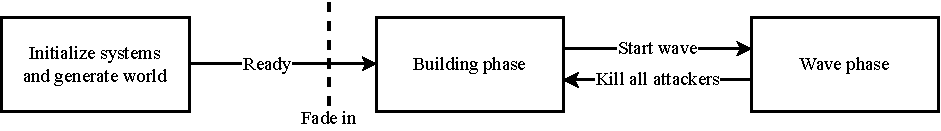
\includegraphics[width=0.8\textwidth]{img/battle scene phases.pdf}
    \caption{\emph{Battle} scene phases.}
    \label{fig:battle-phases}
\end{center}

We will explain the initialization and procedural generation in section~\ref{sec:docs-world-generation}.
In this section, we'll describe only the processes involved in the gameplay.
First we'll explain the game logic, and then the visualizations used to communicate information to the player.

To most systems in involved in the battle, it doesn't matter if the game is currently in the building or wave phase, they behave the same at all times.
Only few things change when a wave starts or ends, which we describe in section~\ref{sec:docs-waves}.

\subsection{Scene contents}\label{sec:docs-battle-scene}

Before we explain what goes on during a battle, we should introduce the contents of the battle scene.
When loaded, the \emph{Battle} scene contains only the UI, and various singleton objects with scripts that each take care of one game system.
We will explain these when they become relevant.

During the procedural generation and initialization, more game objects are created in the scene and various scripts are initialized with data.
For example, the results of the world generation are stored in the \mono{WorldData} singleton script.
The world terrain is created in the scene under the \emph{World} game object, including the obstacle models and visualization of the attacker paths.
Also, an instance of the \emph{Tile} prefab is created for each world tile, and references to the tiles are also stored in \mono{WorldData} script for easy access.
For the rest of this section, we assume the scene is already initialized and ready for the player's inputs.

During the battle, there are also some game objects which persist between scenes and don't originally come from the \emph{Battle} scene.
These are the \mono{SceneController} and \mono{SoundController} we introduced in section~\ref{sec:docs-scripts}.
Additionally, there is \emph{Run Persistence} game object, which contains scripts that persist throughout the player's run.
The only script relevant during battle it has is \mono{RunPersistence}, which keeps track of the player's blueprints and hull.
We will describe it in more detail in section~\ref{sec:docs-run-persistence}.

\subsection{Selecting World Objects}

During the battle, one of the most important things the player can do is to build buildings or use abilities.
To do that, the player first needs to select the blueprint they want to use.
The \mono{SelectionController} keeps track of what objects the player selects or hovers over.
In this subsection, we will illustrate the \mono{SelectionController}'s function by explaining what happens when the player selects objects within the game world.
Selecting and placing blueprints is more complicated, and it will be explained in the next subsection~\ref{sec:docs-place-blueprint}.
The game also visualizes which objects are currently selected or hovered, and it shows additional information on the info panel.
This is ultimately the reason why the player would select a world object.
These visual components will be explained in section~\ref{sec:docs-highlights}, and how the info panel works is described in section~\ref{sec:docs-info-panel}.

In the world, the only selectable objects are tiles and attackers.
When the player selects a building, they have in fact selected the tile the building is built on.
Every frame, the \mono{SelectionController} performs a raycast to determine which selectable object is the cursor over, if any.
The selectable objects have a game objects with a collider on the physics layer \emph{Selection} and a \mono{Selectable} script.
If a selectable world object is hovered over, a reference to its \mono{Selectable} script is saved in the \mono{SelectionController} as currently hovered.
Whenever the currently hovered object changes (even to \emph{null}), the info panel is notified to show information about the hovered object (or to hide).

When the player clicks while an object is hovered, it is selected:
The \mono{selected} field in the \mono{SelectionController} is set to the hovered object and the info panel is notified.
While something is selected, the \mono{SelectionController} still updates which object is hovered.
When the player deselects the object, the field is unset, and again, the info panel are notified.

\subsection{Selecting and Placing a Blueprint}\label{sec:docs-place-blueprint}

Let's start with an example of what happens when from the player's perspective when they place a blueprint:
The player clicks on a blueprint of a tower in the blueprint menu.
It is now selected.
Then, they hover over the tile they want to place the tower on.
The game shows a visualization of the range the tower would have if it was placed there.
We say the selected blueprint is set up as if it was placed there.
Finally, the player clicks to place the tower on the selected tile.

We can see that each of the player's actions had an effect on the state of the selection.
In this section, we'll take a look at what happens in response to each of the player's actions in order to achieve this behavior.
For reference, the possible selection states and action that transition between them are shown in figure~\ref{fig:selection-states}.
Each arrow represents what the player can do in the current state and what is the new state after the action is performed.
Few actions are show with blue arrows instead of black.
These are still actions the player can take, but in the code, they are performed as a deselection followed by a selection.

\begin{center}
    \captionsetup{type=figure}
    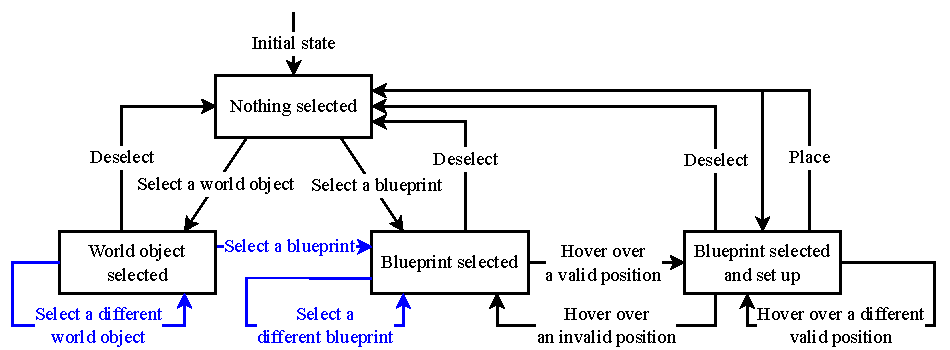
\includegraphics[width=\textwidth]{img/selection states.pdf}
    \caption{Selection states.}
    \label{fig:selection-states}
\end{center}

We have already explained what happens when a world object is selected or deselected, but things are a bit more complicated with blueprints.
We will now explain each of the remaining actions in the diagram.

\head{Selecting a Blueprint}{}
A blueprint can be selected by clicking on it in the blueprint menu user interface (see section~\ref{sec:design-blueprint-menu}) or by pressing a number key on the keyboard that corresponds to its position in the blueprint menu.
Either way, the \mono{SelectionController} gets only the blueprint's index in the blueprint menu.
If this index corresponds to the currently selected blueprint, it gets deselected.
But now, we'll look at what happens when a blueprint gets selected.
During this, the \mono{SelectionController} interacts with other scripts.
Figure~\ref{fig:placing-blueprint} contains a sequence diagram for reference.

First, the \mono{SelectionController} obtains the actual blueprint at the given index from the \mono{BlueprintMenu}.
Then it takes the prefab associated with this blueprint and instantiates it.
Each blueprinted object prefab has on it two scripts that are relevant for us right now:
A script derived from \mono{Placement}, which decides where the blueprint can be placed.
And a script derived from \mono{Blueprinted}, which handles the behavior of the blueprinted object when placed in the world.
For example, the \emph{Budget Sentry} has the script \mono{SimpleBuildingPlacment} for placement and its behavior is implemented by the script \mono{BasicProjectileTower}.

After instantiating the prefab, the \mono{SelectionController} saves a reference to its \mono{Placement} script which signifies that this is the currently selected object.
It then initializes the \mono{Blueprinted} script by giving it a copy of the original blueprint.
Similarly to selecting a world object, it notifies the info panel to show the relevant information.
This is not shown in the sequence diagram to avoid clutter.

\head{Setting Up the Blueprint}{}
We want to accurately preview the effects a blueprint will have, or how it will be affected by other buildings once placed.
To do this, we need to position the blueprinted object in the world as if it actually was placed.
On every update, the \mono{SelectionController} tells the \mono{Placement} to set up the object as if it was placed in the position the player currently hovers over.
The \mono{Placement} returns whether the setup changed from the last frame, and if it did, the \mono{SelectionController} also notifies the \mono{Blueprinted} script.

It is possible that the current position is not a valid placement for the blueprint.
In that case, the \mono{Placement} marks the setup as invalid.
This is represented in figure~\ref{fig:selection-states} as the state \enquote{Blueprint selected}.
However, for the \mono{SelectionController}, there is no distinction between a valid and invalid setup.
From its perspective, the states \enquote{Blueprint selected} and \enquote{Blueprint selected and set up} are just one state.
To the player, they are pretty distinct, because the various visualizations behave differently based on whether the current placement is valid or not, and they communicate the difference to the player.
How these visualizations work is explained in section~\ref{sec:docs-highlights}.

\begin{center}
    \captionsetup{type=figure}
    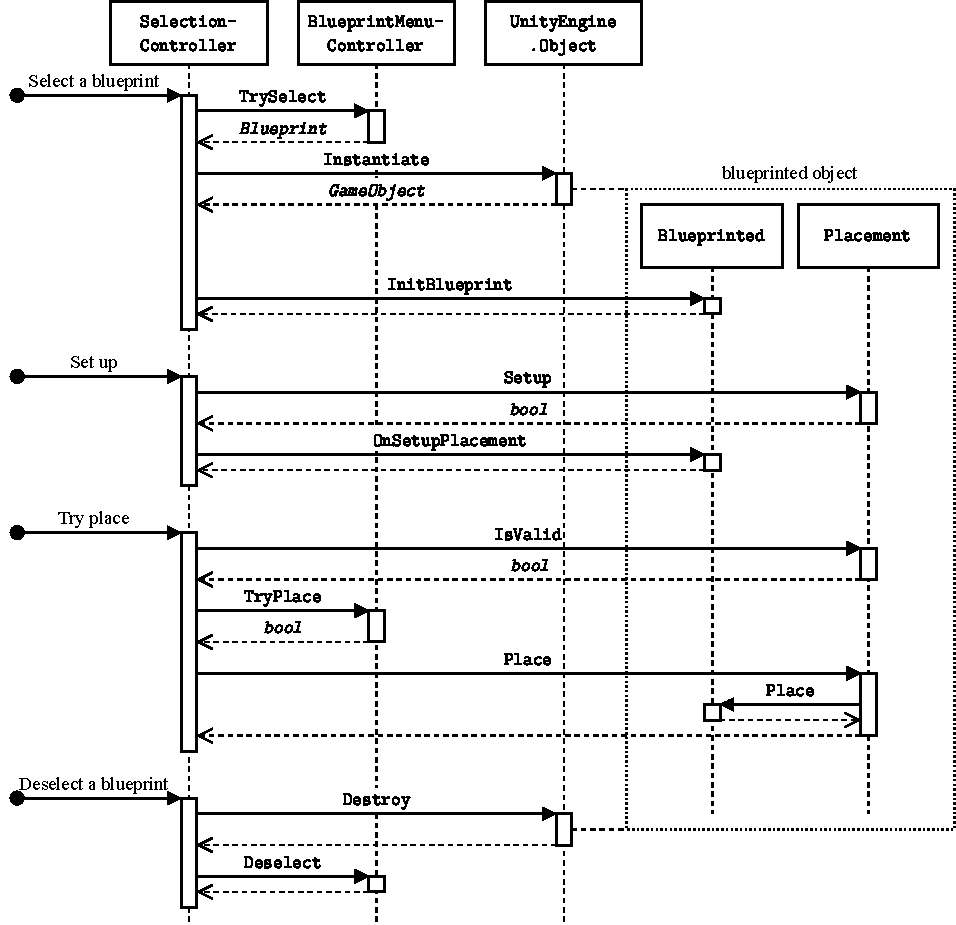
\includegraphics[width=\textwidth]{img/placing a blueprint.pdf}
    \caption{Sequence diagram of events related to placing a blueprint.}
    \label{fig:placing-blueprint}
\end{center}

\head{Placing the Blueprint}{}
When the player clicks to place the selected blueprint, the \mono{SelectionController} first asks the \mono{Placement} if this position is valid.
If it is, the \mono{SelectionController} asks \mono{BlueprintMenu} to try to place the blueprint.
This only means that the \mono{BlueprintMenu} checks if the player can afford the cost and that the blueprint isn't on cooldown.
If this succeeds, the \mono{BlueprintMenu} invokes a command to subtract the cost of the blueprint from the player's resources, and it makes the blueprint go on cooldown if applicable.

If the blueprint cannot be placed, the \mono{SelectionController} just plays an error sound to provide feedback to the player.
Otherwise, it calls the \mono{Place} method on the blueprinted object's \mono{Placement}.
Then the \mono{SelectionController} deselects the blueprint.
However, in figure~\ref{fig:selection-states} the \enquote{Place} action forks and leads to two different states.
This just signifies that after placing an ability, the blueprint gets automatically selected again.

After being actually placed, the \mono{Blueprinted} script enables the visual parts of the blueprinted objects, but the rest is left up to the implementation of the given object.
Usually, their initialization includes registering some modifiers and reactions to modifiable commands (see section~\ref{sec:analysis-modifiable-commands}).
For example, most production blueprints produce resources every turn, so they register a modifier to the modifiable query which determines the production per turn displayed to the player.
They also register a reaction to the event signifying that a wave has ended, because they produce the resources specifically after every wave.

\head{Deselecting the Blueprint}{}
If the selected blueprint gets deselected without placing it, the blueprinted object gets destroyed and the \mono{BlueprintMenu} is notified that the blueprint is no longer selected.
This can also be seen in figure~\ref{fig:selection-states}, but note that the exact sequence of events shown in the diagram is invalid.
It is not possible to deselect a blueprint after it has already been placed.

\head{Hovering over a Blueprint}{}
We would also like to mention how we handle hovering over a blueprint in the blueprint menu, because it is different from hovering over a selectable world object.
In fact, the \mono{SelectionController} doesn't know when the player hovers over a blueprint.
As far as it knows, the player doesn't hover over anything.
The blueprints in the blueprint menu detect the hover on their own and react to the hover accordingly, including notifying the info panel.
The script that makes this work is the \mono{BlueprintDisplay} script on each of the blueprint menu items.
This is done this way, because the blueprint display prefabs are also used in the \emph{Blueprint Selection} scene, where they behave the same.

\subsection{Player State}

Another important singleton script in the \emph{Battle} scene is the \mono{PlayerState}.
Compared to the \mono{SelectionController}, its function is much simpler.
It keeps track of the player's energy, materials and fuel, and if the battle has been won or lost.
Other scripts can use its static modifiable commands to add or spend resources.

Once the fuel amount reached the fuel goal for this level, it invokes its modifiable command \mono{WIN\_LEVEL}.
In reaction to this, the \mono{OverlayController} shows the victory overlay with a button to proceed to the next level.
What happens next is explained in section~\ref{sec:docs-run-persistence}.

\subsection{Attacker Waves}\label{sec:docs-waves}

The \mono{WaveController} script controls what happens during a wave.
It interacts with several other scripts, which we'll describe in the following paragraphs.
For reference, we've lillustrated these interactions in figure~\ref{fig:wave-controller-interactions}.
The diamonds are modifiable commands or events, and for their interactions, we use a convention similar to the diagrams in section~\ref{sec:analysis-modifiable-commands}.

\begin{center}
    \captionsetup{type=figure}
    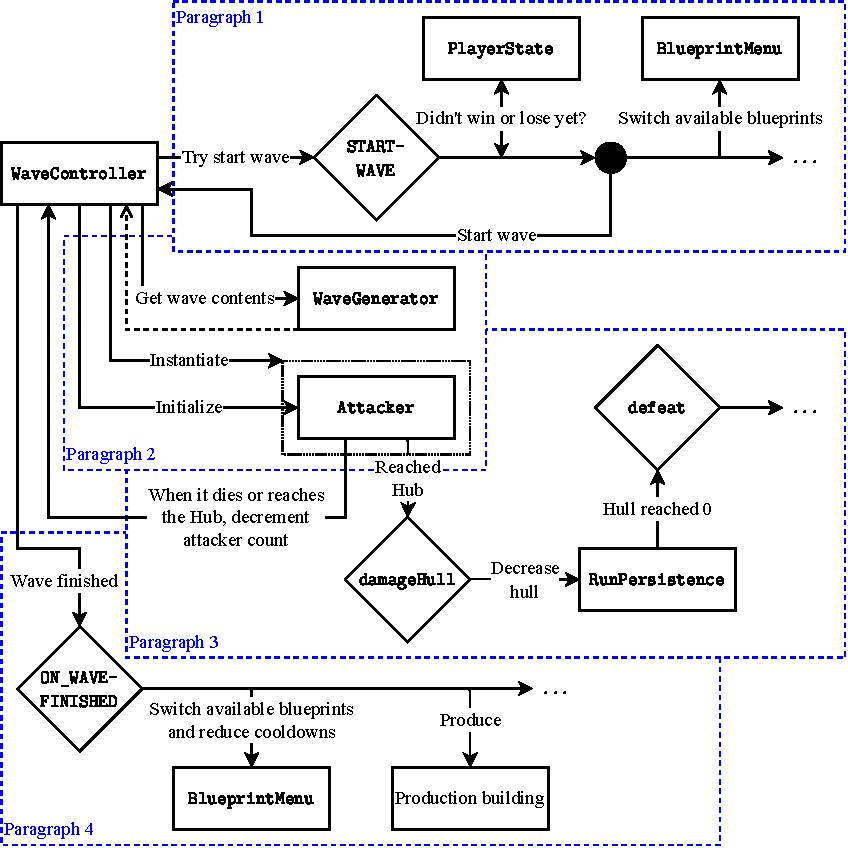
\includegraphics[width=\textwidth]{img/wave controller connections.pdf}
    \caption{Interactions of \mono{WaveController} with other scripts.}
    \label{fig:wave-controller-interactions}
\end{center}

\paragraph*{(1)}
When the player requests to start a new wave, the \mono{WaveController} invokes the \mono{START\_WAVE} modifiable command.
This command has a modifier registered by \mono{PlayerState}, which cancels the command if the battle has been won or lost.
Various scripts react to this command, for example the \mono{BlueprintMenu} changes which blueprints are available from buildings to abilities.

\paragraph*{(2)}
When the wave is started, the \mono{WaveController} requests the contents of the wave from the \mono{WaveGenerator}, and it starts spawning the specified attackers.
To spawn an attacker, it instantiates the prefab specified by the attacker stats, and it initializes the attacker's \mono{Attacker} script.
The attacker then moves and behaves on its own, as implemented in its \mono{Attacker} script.

\paragraph*{(3)}
The \mono{WaveController} does not keep track of the attackers, only their count.
Whenever it spawns an attacker, it increments the count, and whenever an attacker dies or reaches the Hub, the count is decremented.
Once all attackers have been spawned and there are no attackers left in the world, the wave ends, and the \mono{ON\_WAVE\_FINISHED} event is invoked.
This event has many reactions, for example the \mono{BlueprintMenu} switches the blueprint offer back to buildings, and it decrements all cooldowns.
Also, most production buildings produce resources in reaction to \mono{ON\_WAVE\_FINISHED}.

\paragraph*{(4)}
Whenever an attacker reaches the Hub, it invokes the command \mono{damageHull}.
The \mono{RunPersistence} reacts to this and decreases the player's hull.
If the hull reaches 0, the command \mono{defeat} is invoked.
This lets all game systems know that they should stop, and to display the \emph{defeat} overlay.

\subsection{Shooting at Attackers}

During a wave, the towers the player has built shoot at the attackers.
As we described in section~\ref{sec:analysis-targeting}, the towers know that an attacker is in range, if it is within the tower's targeting collider.
They use the \mono{Targeting} script to know which attackers are in range, which attackers are in line of sight, and which attacker they should shoot at, based on the current targeting priority.

A tower's range can be composed of many \mono{TargetingCollider}s, and they can be combined with any set operations to create various range shapes.
Figure~\ref{fig:combining-colliders} shows how we could create a range shaped like a cylinder with a hole.
Whenever an attacker enters or leaves a \mono{TargetingCollider}, it notifies its parent.
Based on the state reported by other children, the parent decided whether to notify its parent.
The scripts that can be children in this targeting tree implement the interface \mono{ITargetingChild} and parents implement \mono{ITargetingParent}.
The root of this tree is the \mono{Targeting} script itself, which uses this information to track which attackers are in range.

\begin{center}
    \captionsetup{type=figure}
    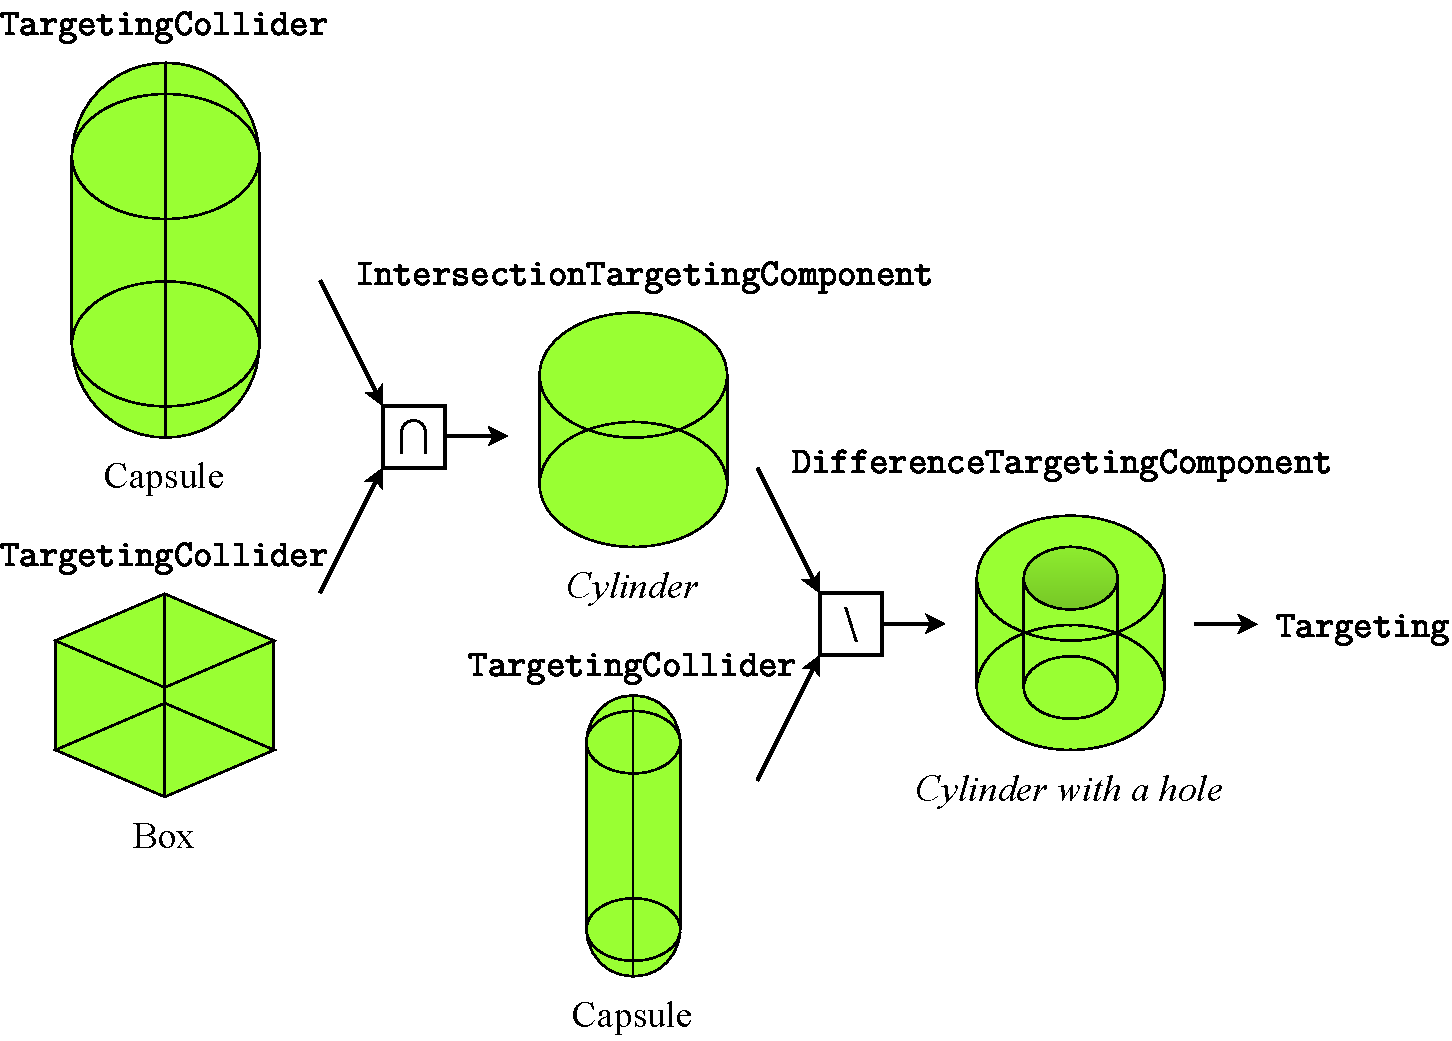
\includegraphics[width=0.8\textwidth]{img/combining colliders.pdf}
    \caption{Combining collider shapes using set operations.}
    \label{fig:combining-colliders}
\end{center}

Most towers ask the \mono{Targeting} every tick they could shoot whether they have a target, and if so, they shoot at it.
Some towers hit their target instantly, but others shoot a projectile, which will take few ticks to hit the target.
Some projectiles might even miss the target.
The behavior of various projectiles is implemented in the derived classes of \mono{Projectile} used in their prefabs.
Once they hit their target, they notify the tower that shot them.

To damage an attacker, the tower should use its method \mono{TryHit}.
The attacker then invokes the \mono{DAMAGE} command, and it also handles this command by decreasing its own HP accordingly.
Similarly, when the player uses an ability to damage attackers, the ability determines its targets, usually using a sphere cast, and damages them via the \mono{TryHit}.
The interactions described in this section are summarized in figure~\ref{fig:shooting}.

\begin{center}
    \captionsetup{type=figure}
    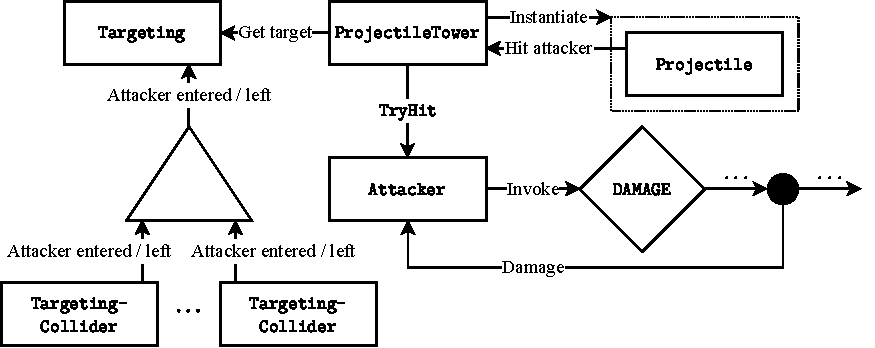
\includegraphics[width=\textwidth]{img/shooting.pdf}
    \caption{Script interactions when a tower shoots at an enemy.}
    \label{fig:shooting}
\end{center}

\subsection{Info Panel}\label{sec:docs-info-panel}

In the following subsections we'll take a look at the more visual elements of the game, whose main job is to communicate information to the player.
We'll start with the info panel.

The info panel exists both in the \emph{Battle} and \emph{Blueprint Selection} scene.
The public methods of its \mono{InfoPanel} script get called directly by various scripts.
To show info about a certain object, the right method is called, and the object is passed as an argument.
The \mono{InfoPanel} saves these references, so it always works with up-to-date information.
The \mono{Hide} method can be used to hide the panel.

To show information about some object, the info panel creates an instance of the corresponding \mono{DescriptionProvider} script.
The \mono{InfoPanel} then asks the \mono{DescriptionProvider} every frame for the current description.
This way, the descriptions can change in real time.
Each \mono{DescriptionProvider} first generates the description with tags as specified in section~\ref{sec:analysis-description-tags}, and then it uses \mono{DescriptionFormatter} to format them into the corresponding formatted text and icons.

Most tags used in the descriptions of buildings or blueprints represent a value that can be modified.
The \mono{Blueprint} script contains a modifiable query for each modifiable value it holds.
The values stored in the blueprint are the base values, and the real up-to-date values are to be obtained through these queries.
For formatting the descriptions, the \mono{DescriptionFormatter} compares these modified values to the base values, and it colors the text based on if the modified value has changed for the better, worse or not at all.

In figure~\ref{fig:description-formatting} we show an example of how a description is produced.
In this case, the info panel is displaying a description of a \emph{Predator} tower, and for that, it has created an instance of a \mono{BlueprintDescriptionProvider}.
In the diagram, the info panel asks the description provider for the description.
The description provider first assembles it from parts provided by the tower and its blueprint, and then it asks the \mono{DescriptionFormatter} to format it.
The \mono{DescriptionFormatter} replaces the tag \enquote{[\$DMG]} with the word \enquote{Damage}, the icon of the damage type, and a colored text with the damage amount.
It reads from the blueprint that in this case, the base damage is 10, and by using the modifiable query \mono{Damage}, it obtains that the current damage should be 17.
So, it outputs that the tower deals 17 damage, and the number is green, because it is greater than the base damage.

\begin{center}
    \captionsetup{type=figure}
    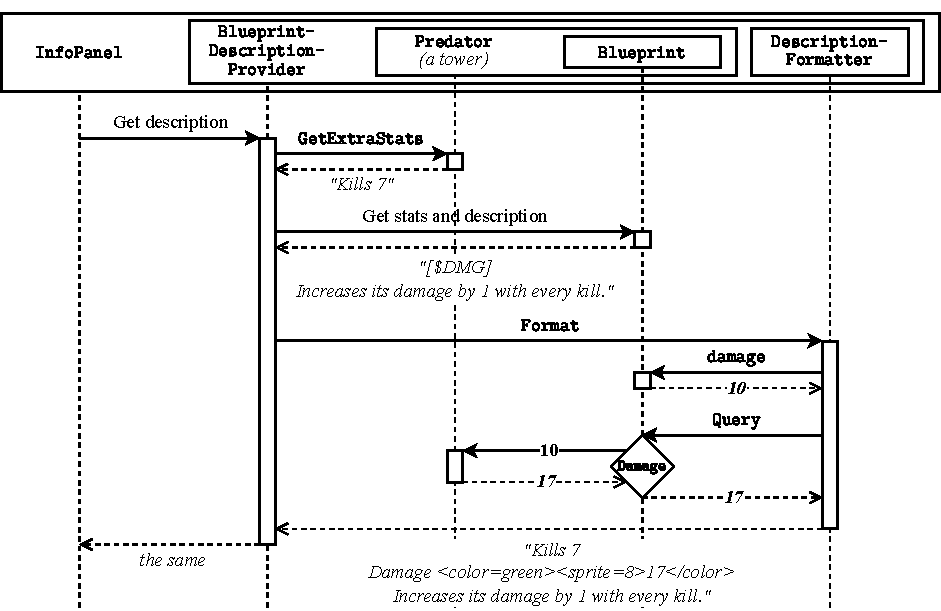
\includegraphics[width=\textwidth]{img/description formatting.pdf}
    \caption{Generating the description to be shown in the info panel.}
    \label{fig:description-formatting}
\end{center}

When a building is selected, the info panel also shows a delete button.
For towers, it also shows arrows that allow the player to change the tower's targeting priority.
Since the info panel has a reference to the building it's displaying information about, it can just directly call the building's public methods for this functionality.
It's important to note that when a building gets destroyed, the building has to unregister all modifiers and reactions it has registered.

\subsection{Visuals and Interpolation}

Scripts that take care of visuals are separated from the game logic.
The visuals scripts have references to the game logic scripts they care about, and they read their public fields, or react to various events.
For example, the scripts that display the player's energy and materials just read the values directly from the \mono{PlayerState} script.
However, sometimes we add some events to the game logic scripts, whose only purpose is to let the visuals know when something happens.
For example, the \mono{SelectionController} has the Unity event \mono{resetVisuals}, which is used to let visuals scripts know that the setup of the blueprint currently being built has changed, so they should reflect this change.

Various visuals scripts also react to the game events.
For example, the \mono{NumberEffects} script spawns a number effect above an attacker whenever the attacker gets damaged, and it creates number effects whenever resources get produced.
These number effects show the amount of damage that was dealt, or the amount and type of the resource produced.

Each blueprinted object also has some scripts that control its visuals.
For example, the script that takes care of the visualization of most projectile-shooting towers is \mono{BasicProjectileTowerVisuals}.
It makes the tower's turret point towards the attacker the tower is targeting, but it also interpolates the rotation to be smooth.
It also subscribes to the tower's \mono{onShoot} Unity event to play an animation when the tower shoots.

We would also like to mention that both attackers and projectiles move the world as a part of the game logic.
Of course, they change their position only 20 times per second, but to the player, their travel needs to look smooth.
So, their visuals scripts simulate their movement in the same way as the game logic scripts, only with a greater temporal resolution.

\subsection{Highlights and Range Visualization}\label{sec:docs-highlights}

When the player selects a building, attacker, or a blueprint, it is highlighted, so the player knows it's selected.
Furthermore, we might highlight other relevant objects differently to show that they are somehow affected by the selected object.
For example, when the player selects a tower, it highlights the attackers in its range in yellow.
We also want to show the affected region of the world, by coloring the terrain accordingly.
For example for towers, we draw their range.
This is described in section~\ref{sec:design-selection-highlights}.

The \mono{HighlightController} looks at the \mono{SelectionController}'s selected and/or hovered objects every frame and determines which objects in the world should be highlighted.
However, each selected object wants to highlight objects differently.
This behavior is implemented in the object's script derived from \mono{HighlightProvider}.
If the selected object has a \mono{HighlightProvider}, or when a selected tile has a building with a \mono{HighlightProvider} on it, the \mono{HighlightController} asks it what objects should be highlighted, and with which color.
It then tells these object to change their highlights accordingly.
The objects that can show highlights implement the interface \mono{IHighlightable}.

The \mono{HighlightController} also closely monitors the \mono{SelectionController} when placing a blueprint.
It highlights the selected tile, or attacker, or it shows just a point highlight which highlights the selected position in the world, based on the blueprinted object's \mono{Placement}.

Each \mono{HighlightProvider} also implements a function that returns the color of the range visualization for any given point, as described in section~\ref{sec:analysis-range}.
The script \mono{RangeVisualization} then creates the range visualization over many frames, based on the \mono{HighlightProvider} that's currently selected according to the \mono{HighlightController}.
The interactions described in this section are shown in figure~\ref{fig:highlights-and-range}.

\begin{center}
    \captionsetup{type=figure}
    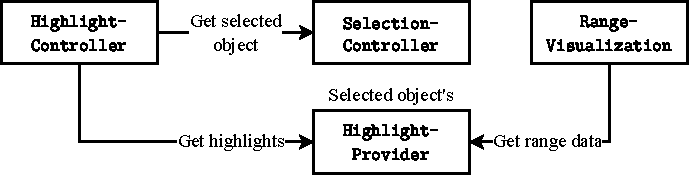
\includegraphics[width=0.9\textwidth]{img/higlights and range.pdf}
    \caption{Interactions between scripts for highlights and range visualization.}
    \label{fig:highlights-and-range}
\end{center}

In addition to our specification in section~\ref{sec:analysis-range}, when placing a blueprint, the \mono{HighlightProvider} also shows in blue the valid positions to place it.
For this, it needs a reference to the given \mono{Placement} script to ask it which positions are valid.

\subsection{Tutorial}

The tutorial is handled by a system separate from other scripts.
It calls their public methods, and modifies their data to achieve the behavior we want.
There are two scripts that handle the tutorial:

\mono{TutorialController} keeps track of the player's progress through the tutorial.
The tutorial is a sequence of steps, and the \mono{TutorialController} has a Unity event for each of them.
At the start of each step, it invokes the corresponding Unity event.
This way, all things that happen during the tutorial can be assigned in the Unity editor.

The script \mono{TutorialActions} then contains methods which do various modifications to various objects within the scene, so these actions can be subscribed to the \mono{TutorialController} Unity events.
\mono{TutorialActions} also contains various checks based on which it tells the \mono{TutorialController} when to go to the next step.

\section{Game Start and Procedural Generation}\label{sec:docs-data}

In this section we'll take a look at the processes that happen from the application start, all the way to generating worlds and waves.
We already described the transitions between scenes in section~\ref{sec:docs-scenes}, and now we'll go into more detail.

\subsection{Loading}

When the application starts, a \enquote{Made with Unity} splash screen is shown, and then the \emph{Loading} scene is loaded.
As we mentioned in section~\ref{sec:docs-scripts}, this scene contains \mono{SceneController} and \mono{SoundController}~--- game objects that persist throughout the entirety of the application runtime and provide useful functionality.
However, the main purpose of this scene is to load various data from the disk into memory.
This is handled by the \mono{StartLoader} script.
We can register to it any number of \mono{ILoader} scripts, which do the loading and store the data in singleton classes.

Currently, the only loader we use is \mono{TerrainTypeLoader}, which loads the terrain types from the \emph{StreamingAssets/TerrainTypes} folder.
For each terrain type file, the \mono{TerrainTypeLoader} creates a new \mono{TerrainType} object using the function \mono{Parse} it has.
The parsing is done using a simple parser implemented in the folder \emph{Scripts/Data/Parsers}.
The terrain type file format is described in section~\ref{sec:docs-terrain-type}.

\subsection{Menus and Starting a Run}

The \emph{Menu} scene contains mostly just three buttons and an object with the \mono{RunStarter} script.
All three buttons call a method on the \mono{RunStarter} when pressed.
When the \enquote{Start} button is pressed, the \mono{RunStarter} instantiates the \emph{RunPersistence} prefab, configures it, and calls the \mono{NextLevel()} method on its \mono{RunPersistence} script.

Pressing the \enquote{Custom Run} button takes the player to the \emph{Run Settings} scene.
It contains more UI elements, and another object with a \mono{RunStarter} script.
Here, the player can change the run settings by interacting with the UI elements, which in turn notify the \mono{RunStarter} about these changes.
When the player starts the run, the instantiated \emph{RunPersistence} prefab is then configured according to the settings.
If the \enquote{Select starting blueprints} option is enabled, instead of going to the first level, the scene \emph{Blueprint Selection} is loaded, where the player can select the starting blueprints.

\subsection{Run Persistence and Blueprint Rewards}\label{sec:docs-run-persistence}

The \emph{RunPersistence} object persists between scenes, and it only destroys itself when a run ends.
It holds all scripts that need to remember some state throughout the whole run:
The \mono{RunPersistence} script keeps track of the player's hull and blueprints, the run seed, the current level, and it gives orders to the other scripts.
The \mono{BlueprintRewardController} script generates blueprint rewards for the player.

After the player beats a level, the \mono{RunPersistence} asks the \mono{BlueprintRewardController} to reward the player with blueprints.
For the rewards after the first tutorial level, the \mono{BlueprintRewardController} has a predefined blueprint selection, but for normal blueprint rewards, it picks the selection randomly, based on its seed.
It then changes the scene to the \emph{Blueprint Selection} scene, and initializes the \mono{BlueprintSelectionController} script in it with the selection.

The \mono{BlueprintSelectionController} handles the blueprint selection.
It initializes the scene by instantiating \emph{BlueprintDisplay} prefabs which depict the blueprints on offer and the player's current collection.
When the player clicks on one of the blueprints, it notifies the \mono{BlueprintSelectionController}, which handles the selection logic.
It also modifies the blueprints' outlines to communicate to the player what is selectable or selected, and it makes the info panel show relevant information.
Once the player confirms their selection by clicking on a button, it returns what the player chose in a callback to the \mono{RunPersistence}, which updates the player's blueprint collection and proceeds to the next level.

The interactions described in this section are summarized in figure~\ref{fig:blueprint-selection}.
\begin{center}
    \captionsetup{type=figure}
    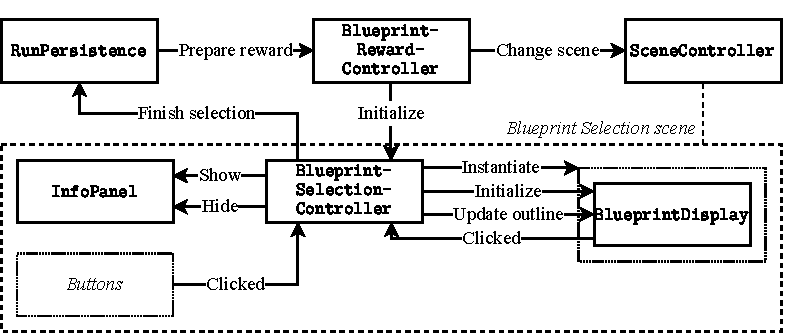
\includegraphics[width=\textwidth]{img/blueprint selection.pdf}
    \caption{Interactions between scripts during blueprint selection.}
    \label{fig:blueprint-selection}
\end{center}

\subsection{Seed Branching and Level Initialization}\label{sec:docs-level-init}

As we described in section~\ref{sec:analysis-rng}, we use \emph{seed branching} everywhere throughout the procedural generation.
This means that whenever some system needs an RNG, it gets a seed from another system, and from this seed it creates its own RNG instance to use.
Figure~\ref{fig:seed-branching} shows how the seeds get propagated across the game's systems.
When starting a new run, the \mono{RunStarter} creates a new instance of \mono{RunPersistence}, and it is given a run seed.
It is either randomly generated using \mono{System.Random} or selected by the player.
The \mono{RunPersistence} then initializes the \mono{BlueprintRewardController}, giving it a seed to generate rewards from.

Whenever a new level is started, the \mono{WorldGenerator} in the \emph{Battle} scene finds the \mono{RunPersistence} and asks it to set up the level settings.
For this, the \mono{RunPersistence} uses the \mono{LevelSetter} script, which finds the relevant scripts in the scene and sets them up.
The \mono{RunPersistence} generates a seed for the \mono{LevelSetter}.
The \mono{LevelSetter} generates a new seed for the world generator and configures the number of paths and their lengths, based on the level number, storing this information in the \mono{WorldSettings} script.
It also configures the \mono{WaveGenerator}'s seed and parameters, and the fuel goal in the \mono{PlayerState}.
Figure~\ref{fig:seed-branching} shows the \mono{WorldSettings} and \mono{WaveGenerator} multiple times, to convey that each level has a new instance of these scripts.

\begin{center}
    \captionsetup{type=figure}
    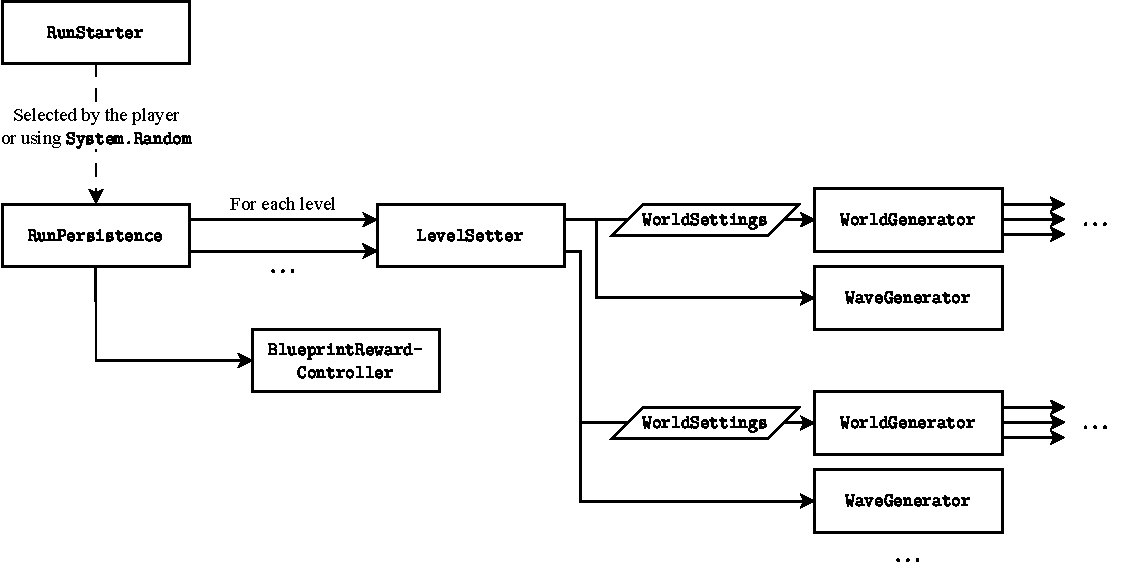
\includegraphics[width=\textwidth]{img/seed splitting.pdf}
    \caption{Seed propagation using seed branching.}
    \label{fig:seed-branching}
\end{center}

\subsection{Procedural World Generation}\label{sec:docs-world-generation}

The \mono{WorldGenerator} handles the world generation by giving orders to other scripts.
We illustrate its interactions with other scripts in figure~\ref{fig:world-generator}.
As we mentioned, when the \emph{Battle} scene is loaded, it asks the \mono{RunPersistence} to set up the level.
All information the \mono{WorldGenerator} needs is supplied through the \mono{WorldSettings} script.
The world generator then reads the information, and calls other generator scripts, which each take care of one stage of the world generation, as described in section~\ref{sec:analysis-procedural-generation}.

\begin{center}
    \captionsetup{type=figure}
    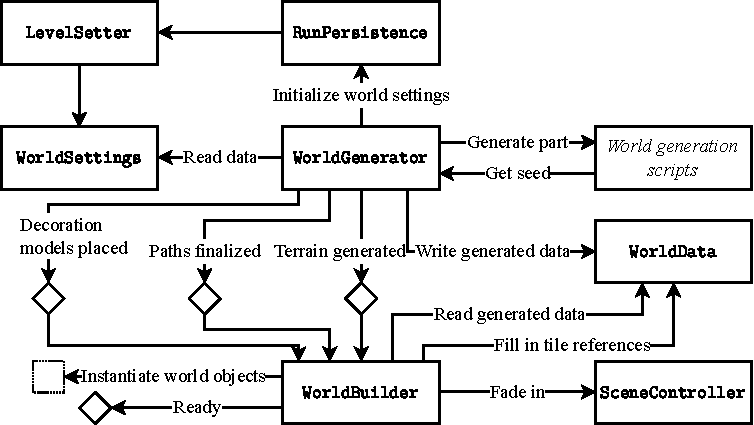
\includegraphics[width=\textwidth]{img/world generator.pdf}
    \caption{Script interactions during world generation.}
    \label{fig:world-generator}
\end{center}

In order of use, the world generation scripts are:
\begin{enumerate}
    \item \mono{PathEndPointPicker} picks path end points (section~\ref{sec:analysis-path-starts}).
    \item \mono{PathPlanner} generates main paths (section~\ref{sec:analysis-main-paths}).
    \item \mono{WFCGenerator} generates the terrain (section~\ref{sec:analysis-terrain-generation}).
    \item \mono{ObstacleGenerator} selects the positions for obstacles (section~\ref{sec:analysis-obstacles}).
    \item \mono{PathFinalizer} then creates the final path network (section~\ref{sec:analysis-final-paths}).
    \item \mono{ObstacleModelScatterer} selects the obstacle model positions and sizes (section~\ref{sec:analysis-obstacles}).
\end{enumerate}

The \mono{WorldGenerator} gives each script the information it needs, be it from the \mono{WorldSettings} or data that was generated in some previous stage.
All the algorithms are randomized, and they can require multiple random number generators.
To generate seeds for their RNG's, they use the \mono{WorldGenerator}'s RNG that was initialized with the seed from \mono{WorldSettings}.
After each stage, the \mono{WorldGenerator} writes the generated data into the \mono{WorldData} script.
From the \mono{WorldData}, other scripts can read the information about the generated world, as also mentioned in section~\ref{sec:docs-battle-scene}.
After several stages, the \mono{WorldGenerator} invokes an event to notify other scripts that new world data is ready.

The world generation stages are done in background threads so that the game doesn't become unresponsive.
however, in Unity, we cannot instantiate objects from a background thread.
The script \mono{WorldBuilder} reacts to the \mono{WorldGenerator}'s events, and it builds the terrain, obstacles, paths, and tiles in the main thread.
It also reads the world data from the \mono{WorldData} script, and writes back references to the tile instances it created.

Creating many objects is expensive, so to prevent stuttering, we use Unity coroutines to build the world across multiple frames.
Currently, the screen is faded out using the \mono{SceneController} during world generation, but later we'd like to add an animation, which would make any stutters obvious.
Once the \mono{WorldBuilder} finishes building the world, it tells the \mono{SceneController} to fade in the screen, and it invokes an event to notify all other scripts that the world is generated.